\section{Input Assembly}

\subsection{Overview}
\begin{frame}{Input Assembly Stage}
  \begin{columns}
    \begin{column}{0.5\textwidth}
      \small
      \begin{raybox}{Input Assembly}
        \textbf{Input:} Vertex data from application \\
        \textbf{Output:} Organized vertex streams for vertex shader

        \vspace{0.3cm}
        \textbf{Purpose:}
        \begin{itemize}
          \item Pull vertex data from memory
          \item Organize data into vertex attributes
          \item Handle indexed vs non-indexed drawing
          \item Set up primitive topology
        \end{itemize}
      \end{raybox}
    \end{column}
    \begin{column}{0.5\textwidth}
      \begin{tikzpicture}[scale=1]
        % Memory representation
        \node[rectangle, draw, fill=LightGray, minimum width=2cm, minimum height=0.4cm] (mem1) at (0,3) {\tiny Position Data};
        \node[rectangle, draw, fill=LightGray, minimum width=2cm, minimum height=0.4cm] (mem2) at (0,2.4) {\tiny Normal Data};
        \node[rectangle, draw, fill=LightGray, minimum width=2cm, minimum height=0.4cm] (mem3) at (0,1.8) {\tiny UV Data};
        \node[rectangle, draw, fill=LightGray, minimum width=2cm, minimum height=0.4cm] (mem4) at (0,1.2) {\tiny Index Data};

        \draw[->, thick, PrimaryColor] (1.2,2) -- (2.5,2);

        % Assembled vertex
        \node[rectangle, draw, fill=ObjectColor!20, minimum width=1.5cm, minimum height=1.5cm] (vertex) at (3.5,2) {
          \begin{minipage}{1.3cm}
            \centering
            \tiny
            \textbf{Vertex} \\
            Position \\
            Normal \\
            UV \\
            Color
          \end{minipage}
        };

        \node[below] at (0,0.8) {\scriptsize Vertex Buffers};
        \node[below] at (3.5,0.8) {\scriptsize Assembled Vertex};
      \end{tikzpicture}
    \end{column}
  \end{columns}
\end{frame}

\subsection{Vertex Data}
\begin{frame}{Vertex Attributes}
  \begin{columns}
    \begin{column}{0.5\textwidth}
      \begin{conceptbox}{Common Vertex Attributes}
        \begin{itemize}
          \item \textbf{Position:} 3D coordinates (vec3)
          \item \textbf{Normal:} Surface normal vector (vec3)
          \item \textbf{Texture Coordinates:} UV mapping (vec2)
          \item \textbf{Color:} Vertex color (vec3/vec4)
        \end{itemize}
      \end{conceptbox}
    \end{column}
    \begin{column}{0.5\textwidth}
      \begin{mathbox}{Vertex Layout Example}
        \small
        \begin{align}
          \text{Vertex} =
          \begin{cases}
            \text{Position:} & (x, y, z) \\
            \text{Normal:} & (n_x, n_y, n_z) \\
            \text{UV:} & (u, v) \\
            \text{Color:} & (r, g, b, a)
          \end{cases}
        \end{align}

        \vspace{0.2cm}
        \textbf{Total size:} 3 + 3 + 2 + 4 = 12 floats = 48 bytes
      \end{mathbox}
    \end{column}
  \end{columns}

  \vspace{0.3cm}

  \begin{tikzpicture}
    \node[rectangle, draw, fill=PrimaryColor!20, minimum width=1.2cm, minimum height=0.6cm] (pos) at (0,0) {\tiny Position};
    \node[rectangle, draw, fill=SecondaryColor!20, minimum width=1.2cm, minimum height=0.6cm] (norm) at (1.5,0) {\tiny Normal};
    \node[rectangle, draw, fill=AccentColor!20, minimum width=0.8cm, minimum height=0.6cm] (uv) at (2.9,0) {\tiny UV};
    \node[rectangle, draw, fill=ObjectColor!20, minimum width=1.2cm, minimum height=0.6cm] (col) at (4.1,0) {\tiny Color};

    \node[below] at (0,-0.5) {\scriptsize 12 bytes};
    \node[below] at (1.5,-0.5) {\scriptsize 12 bytes};
    \node[below] at (2.9,-0.5) {\scriptsize 8 bytes};
    \node[below] at (4.1,-0.5) {\scriptsize 16 bytes};
  \end{tikzpicture}
\end{frame}

\subsection{Primitive Types}
\begin{frame}{Primitive Topology}
  \begin{columns}
    \begin{column}{0.6\textwidth}
      \begin{raybox}{Primitive Types}
        \textbf{Points:} Individual vertices
        \begin{itemize}
          \item Used for particle systems
          \item Point sprites
        \end{itemize}

        \vspace{0.2cm}
        \textbf{Lines:} Connected line segments
        \begin{itemize}
          \item Wireframe rendering
          \item Debug visualization
        \end{itemize}

        \vspace{0.2cm}
        \textbf{Triangles:} Most common primitive
        \begin{itemize}
          \item Standard for 3D surfaces
          \item Hardware optimized
        \end{itemize}
      \end{raybox}
    \end{column}
    \begin{column}{0.4\textwidth}
      \begin{tikzpicture}[scale=1]
        % Points
        \node at (0,3.5) {\textbf{Points}};
        \foreach \i in {0,1,2} {
          \fill[PrimaryColor] (\i*0.5,3) circle (2pt);
        }

        % Lines
        \node at (0,2.3) {\textbf{Lines}};
        \draw[thick, SecondaryColor] (0,2) -- (0.5,2) -- (1,1.8) -- (1.5,2.2);
        \foreach \x/\y in {0/2, 0.5/2, 1/1.8, 1.5/2.2} {
          \fill[SecondaryColor] (\x,\y) circle (2pt);
        }

        % Triangles
        \node at (0,1.1) {\textbf{Triangles}};
        \draw[thick, ObjectColor, fill=ObjectColor!20] (0,0) -- (0.8,0) -- (0.4,0.75) -- cycle;
        \draw[thick, ObjectColor, fill=ObjectColor!20] (0.8,0) -- (1.6,0) -- (1.2,0.75) -- cycle;
      \end{tikzpicture}
    \end{column}
  \end{columns}
\end{frame}

\subsection{Drawing Methods}
\begin{frame}{Indexed vs Non-Indexed Drawing}
  \footnotesize
  \begin{columns}
    \begin{column}{0.5\textwidth}
      \begin{conceptbox}{Non-Indexed Drawing}
        \textbf{Direct vertex specification}

        Each vertex is specified multiple times for shared vertices.

        \vspace{0.2cm}
        \textbf{Problem:}
        \begin{itemize}
          \item Vertex duplication
          \item Increased memory usage
          \item Inefficient for complex meshes
        \end{itemize}
      \end{conceptbox}
    \end{column}
    \begin{column}{0.5\textwidth}
      \begin{mathbox}{Indexed Drawing}
        \textbf{Vertices referenced by indices}
        Each vertex is stored once, and indices specify how to connect them.

        \vspace{0.2cm}
        \textbf{Benefits:}
        \begin{itemize}
          \item No vertex duplication
          \item Lower memory usage
          \item Vertex cache friendly
        \end{itemize}
      \end{mathbox}
    \end{column}
  \end{columns}

  \vspace{0.3cm}

  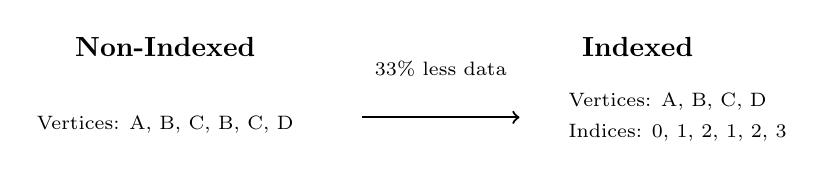
\begin{tikzpicture}
    % Non-indexed example
    \node at (0,1.5) {\textbf{Non-Indexed}};
    \node[align=left] at (0,0.5) {\scriptsize Vertices: A, B, C, B, C, D};

    % Indexed example
    \node at (6,1.5) {\textbf{Indexed}};
    \node[align=left, anchor=west] at (5,0.8) {\scriptsize Vertices: A, B, C, D};
    \node[align=left, anchor=west] at (5,0.4) {\scriptsize Indices: 0, 1, 2, 1, 2, 3};

    \draw[->, thick] (2.5,0.6) -- (4.5,0.6);
    \node[above] at (3.5,1) {\scriptsize 33\% less data};
  \end{tikzpicture}
\end{frame}
